% Appendix 11: The Form-Constancy Mechanism and Portrait Painting
% Source pages: 286–287

\chapter{The Form-Constancy Mechanism and Portrait Painting}

The well-known artistic effect by which the person depicted in a portrait ``follows the
viewer with his eyes'' as the viewer moves can be amplified, so that the portrait begins
to ``turn with its whole body'' within the frame in pursuit of the viewer.  Such mobility
of the depicted person can be explained by the action of the form-constancy mechanism.

Fig.\,11.1 shows a schematic representation (view from above) of a portrait~$b$ hanging
on wall~$a$.  When the viewer occupies position~$A$, i.e.\ his gaze makes a right angle
with the plane of the picture (and of the wall), he sees the image as the artist created
it.  When the viewer moves to position~$B$ or~$C$, his gaze makes an acute angle~$\alpha$
with the plane of the wall and picture.  In this case the retinal image of the picture is
strongly distorted compared with that corresponding to position~$A$.

\begin{figure}[H]
    \centering
    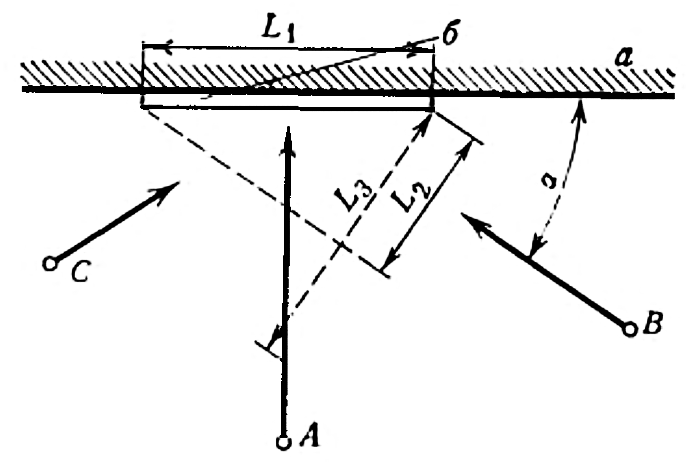
\includegraphics[width=0.6\linewidth]{figures/f11.1.png}
\end{figure}
\figblock{11.1}{View from above.  Portrait~$b$ hangs on wall~$a$.  At position~$A$ the
  gaze is normal to the picture plane.  At position~$B$ or~$C$ the gaze makes acute
  angle~$\alpha$ with the wall; the form-constancy mechanism ``stretches'' the retinal
  image horizontally from width~$b_1$ to~$b_3$, effectively rotating the depicted person
  to face the viewer.}

Since every person has excellent knowledge of the ``geometry'' of a human face, its
distortion due to the deviation of~$\alpha$ from a right angle is immediately
subconsciously compensated by the form-constancy mechanism: this mechanism as it were
``stretches'' the retinal image of the picture horizontally to the width~$b_3$ at which
the face appears in its usual form.  Clearly $b_3 \gg b_1$.  Taken together, this effect
leads to an apparent rotation of the whole image perpendicular to the line of sight from
point~$B$.

\srcpage{287}

Now consider the transformation of the appearance of wall~$a$.

If the system of wall~$a$ and portrait~$b$ is observed simultaneously, two cases are
possible.  If the picture frame is perceived as an element of the picture itself, the
form-constancy mechanism simply allows looking at the picture at sufficiently acute
angles~$\alpha$.  In those (comparatively rare) cases where the artist succeeds in
``uncoupling'' the portrait from the frame---making the frame be subconsciously perceived
as part of the wall rather than of the picture---the described ``rotations'' of the image
will be perceived as rotations relative to the picture frame, and the portrait will
``follow'' the viewer not only with the eyes but through apparent turns of the face and
body relative to the frame.

The question of what artistic means allow one to ``uncouple'' portrait from frame is not
considered here.  We note only that the apparent rotation is impeded by a frontal
depiction of the sitter, in which the line of the shoulders is parallel to the picture
plane: this as it were ``anchors'' the sitter to the picture plane defined by the frame.
In those cases where the artist places the sitter so that his shoulder line is
approximately perpendicular to the picture plane, and simultaneously removes everything
that might ``anchor'' the depicted person to that plane, the effect of ``rotations'' of
the portrait relative to the frame is very easily observed.  The described property is
possessed by such portraits as the \emph{Lady with an Ermine} by Leonardo da Vinci and
many others.

If one limits oneself to the collection of the State Tretyakov Gallery alone, one may
cite the portrait of Baryatinsky by Rokotov, the portrait of Derzhavina by Borovikovsky,
the portraits of Rostopchina by Kiprensky and of Putyatina by Venetsianov.  The same
property belongs to Tropinin's painting \emph{Boy with a Zhaleika} and to a number of
other works.
